\section{NLP}

Natural Language Processing \ac{NLP} ist eine Technologie, mit der Texte oder Sprache in strukturierte Informationen codiert werden kann. Sie vereint die Forschungsgebiete künstliche Intelligenz in der Computerwissenschaft und Linguistik (\cite[vgl.][1]{ITWISSEN}). Ziel ist es, einem maschinenlesbaren Text die richtige Bedeutung zuzuordnen. 
Der klassischen Ansatz des \ac{NLP} untergliedert en Analyseprozess in eigenständige Unteraufgaben, die sequenziell abgearbeitet werden.

\begin{wrapfigure}{r}{8cm}

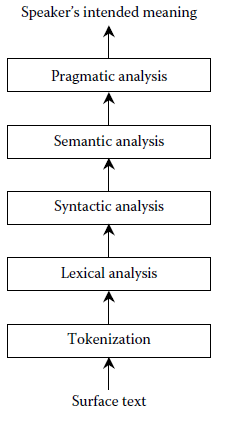
\includegraphics[width=8cm]{pictures/Analyseschritte.png}
\caption{Analyseschritte im klassischen NLP nach \cite[vgl.][4]{DALE}}
\label{fig:STEPS}
\end{wrapfigure}


Die Abbildung \ref{fig:STEPS} zeigt die einzelnen Schritte der Textanalyse nach nach Dale. Den ersten Schritt bildet die \textit{Tokenization}. Zur Vorbereitung des Textes auf die weiteren Analyseschritte werden fundamentale Textbausteine, also Wörtern und Sätzen identifiziert. In segmentierten Sprachen wie dem Englischen, wird das \textit{White-Space-Zeichen} zum separieren der einzelnen Worte genutzt. Komplexe Probleme in diesem Zusammenhang sind beispielsweise die richtige Interpretation der Rolle eines Punktes (Satzende, Abkürzung oder Nummerntrennzeichen), der Umgang mit Mehrwortbenennungen oder die Normalisierung des Textes (Vereinheitlichung von unterschiedlicher Schreibweisen eines Wortes). Hierbei ist die Aussagekraft des Wort- oder Satzkontextes nicht zu unterschätzen. Für die Implementierung der Tokenization existieren zahlreiche regelbasierte Ansätze.

Die lexikalische Analyse analysiert den Text auf Ebene des einzelnen Wortes. Ein Wort bezeichnet hierbei eine Sammlung von Zeichenfolgen, die zu einem Lemma (Grundform) gehören. Im Rahmen der lexikalischen Analyse wird also eine Zeichenfolge (z.B. singt) in ein Lemma mit morphologischen Zusatzinformationen (z.B. SINGEN, 3. Person Singular Präsens) zugeordnet. Im Vergleich zu anderen Sprachen, in denen durch Flexion zahlreiche komplexe Wortformen entstehen, ist diese Aufgabe im Englischen vergleichsweise einfach. Es stehen außerdem umfangreiche lexikale Ressourcen für die lexikalische Analyse zur Verfügung.












